%%%%%%%%%%%%%%%%%%%%%%%%%%%%%%%%%%%%%%%%%%%%%%%%%%%%%%%%%%%%%%%%%%
%%%%%%%%%%%%%%%%%%%%%%%%%%%%%%%%%%%%%%%%%%%%%%%%%%%%%%%%%%%%%%%%%%
\chapter{Zuverlässige und reproduzierbare Datenauswertung}
\label{sec:manage}
%%%%%%%%%%%%%%%%%%%%%%%%%%%%%%%%%%%%%%%%%%%%%%%%%%%%%%%%%%%%%%%%%%
%%%%%%%%%%%%%%%%%%%%%%%%%%%%%%%%%%%%%%%%%%%%%%%%%%%%%%%%%%%%%%%%%%

R bietet viele Möglichkeiten, die dabei helfen, Datenauswertungen zuverlässig und reproduzierbar zu machen. Dazu gehört es, mit automatisierbaren Befehlsskripten zu arbeiten (Abschn.\ \ref{sec:scripting}). In den vergangenen Jahren ist zunehmend auch die Integration von Datenanalyse und schriftlicher Dokumentation in einem gemeinsamen Dokument in den Fokus gerückt (Abschn.\ \ref{sec:rmd}). Besondere Lösungen sind notwendig, um ein hohes Niveau an exakter Reproduzierbarkeit der Ergebnisse herstellen zu können (Abschn.\ \ref{sec:reproducibility}).

%%%%%%%%%%%%%%%%%%%%%%%%%%%%%%%%%%%%%%%%%%%%%%%%%%%%%%%%%%%%%%%%%%
%%%%%%%%%%%%%%%%%%%%%%%%%%%%%%%%%%%%%%%%%%%%%%%%%%%%%%%%%%%%%%%%%%
\section{Befehlssequenzen im Editor bearbeiten}
\label{sec:scripting}
%%%%%%%%%%%%%%%%%%%%%%%%%%%%%%%%%%%%%%%%%%%%%%%%%%%%%%%%%%%%%%%%%%
%%%%%%%%%%%%%%%%%%%%%%%%%%%%%%%%%%%%%%%%%%%%%%%%%%%%%%%%%%%%%%%%%%

Für Datenanalysen, die über wenige Teilschritte hinausgehen, ist eine interaktive Arbeitsweise direkt auf der Konsole nicht sinnvoll. Stattdessen lässt sich die Auswertung automatisieren, indem alle Befehle zunächst zeilenweise in eine als \emph{Skript} bezeichnete Textdatei geschrieben werden, die dann ihrerseits von R komplett oder in Teilen ausgeführt wird.

\index{Skript}\index{Editor}\index{Befehlsskript|see{Skript}}
Um Befehlsskripte zu erstellen, bietet RStudio (Abschn.\ \ref{sec:gui}) einen Texteditor, der sich über den Menüeintrag \emph{File} \textrightarrow\ \emph{New File} \textrightarrow\ \emph{R Script} öffnen lässt und daraufhin bereit für die Eingabe von Befehlszeilen ist. Der Texteditor erstellt automatisch zu jeder öffnenden Klammer eine passende schließende und hebt R-Befehle farblich hervor (\emph{syntax-highlighting}). Mit der\index{Tastaturkurzel@Tastaturkürzel} Tastenkombination \myURL{Strg+Return} wird der Befehl in derjenigen Zeile von R ausgeführt, in der sich die Eingabemarke gerade befindet (icon \emph{Run}). Um in einem Schritt mehrere Befehlszeilen auswerten zu lassen, markiert man diese und führt sie ebenfalls mit \myURL{Strg+Return} aus. Um das komplette Skript ausführen zu lassen, kann das icon \emph{Source} verwendet werden. Verursacht einer der auszuführenden Befehle eine Fehlermeldung, unterbricht dies die Verarbeitung nicht. Folgende Befehle werden dann also trotzdem ausgewertet. Einfache Warnungen werden gesammelt am Schluss aller Ausgaben genannt. Befehlsskripte lassen sich über den Menüeintrag \emph{File} \textrightarrow\ \emph{Save As\ldots} speichern und über \emph{File} \textrightarrow\ \emph{Open File\ldots} laden.

In externen Dateien gespeicherte Skripte lassen sich in der Konsole mit \lstinline!source("<<Dateiname>>")!\index[func]{source()@\lstinline{source()}} in einem Schritt komplett einlesen, wobei R die enthaltenen Befehle ausführt.\footnote{Es ist nicht notwendig, R im interaktiven Modus zu starten, um ein Befehlsskript ausführen zu lassen, dafür existiert auch ein\index{Batch-Modus} \emph{Batch-Modus}, vgl.\ \lstinline!?Rscript!.} Befindet sich die Skriptdatei nicht im aktiven Arbeitsverzeichnis, muss der vollständige Pfad zum Skript zusätzlich zu seinem Namen mit angegeben werden, z.\,B.\ \lstinline!source("c:/work/r/skript.R")!.\footnote{Wird das einzulesende Skript nicht gefunden, ist zunächst mit \lstinline!dir()!\index[func]{dir()@\lstinline{dir()}} zu prüfen, ob das von R durchsuchte Verzeichnis (ohne explizite Angabe eines Pfades ist es das mit \lstinline!getwd()! angezeigte Arbeitsverzeichnis) auch tatsächlich das Skript enthält.} Wird dabei das Argument \lstinline!echo=TRUE! gesetzt, werden die im Skript enthaltenen Befehle selbst mit auf der Konsole ausgegeben, andernfalls erscheint nur die Ausgabe dieser Befehle. Gegenüber der interaktiven Arbeitsweise bieten Skripte u.\,a.\ folgende Vorteile:

\begin{itemize}
\item Der Überblick über alle auszuführenden Befehle wird erleichtert, zudem können die Auswertungsschritte vorgeplant bzw.\ später gedanklich nachvollzogen werden.
\item Teilschritte komplexer Auswertungen können einzeln nacheinander oder in größeren Blöcken ausgeführt werden, um Zwischenergebnisse auf ihre Richtigkeit zu prüfen.
%\item Man kann ein einmal erstelltes Skript immer wieder ausführen, anpassen und erweitern. Dies ist etwa bei nachträglichen Veränderungswünschen an Grafiken hilfreich: Anders als z.\,B.\ in Programmen zur Tabellenkalkulation müssen so im Fall von anderen Überschriften oder Achsenskalierungen nicht viele schon bestehende Grafiken mit immer denselben Schritten einzeln geändert werden. Stattdessen reicht es aus, das Skript einmal zu ändern und neu auszuführen, um die angepassten Grafiken zu erhalten.
\item Ein für die Auswertung eines Datensatzes erstelltes Skript lässt sich häufig mit nur geringen Änderungen für die Analyse anderer Datensätze anpassen und erweitern. Diese Wiederverwendbarkeit einmal geleisteter Arbeit ist bei rein grafisch zu bedienenden Programmen nicht gegeben und spart auf längere Sicht Zeit. Zudem vermeidet eine solche Vorgehensweise Fehler, wenn bewährte Befehlssequenzen eingesetzt werden.
\item Ein erstelltes Skript dokumentiert gleichzeitig die Auswertungsschritte und unterstützt damit die Reproduzierbarkeit der gewonnenen Ergebnisse statistischer Analysen (Abschn. \ref{sec:reproducibility}).
\item Skripte lassen sich zusammen mit dem Datensatz, für dessen Auswertung sie gedacht sind, an Dritte weitergeben. Neben dem Aspekt der so möglichen Arbeitsteilung kann die Auswertung von anderen Personen nachvollzogen und kontrolliert werden. Dies ist i.\,S.\ einer größeren Auswertungsobjektivität sinnvoll.\footnote{Da R mit\index[func]{shell()@\lstinline{shell()}} \lstinline!shell()! auch auf Funktionen des Betriebssystems zugreifen kann, sollten aus Sicherheitsgründen nur geprüfte Skripte aus vertrauenswürdiger Quelle ausgeführt werden.}
\item Es\index[func]{"\#@\texttt{\#}} lassen sich von R nicht als Befehl interpretierte Kommentare einfügen, z.\,B.\ um die Bedeutung der Befehlssequenzen zu erläutern. Kommentare\index{Kommentar} sind dabei alle Zeilen bzw.\ Teile von Zeilen, die mit einem \lstinline!#! Symbol beginnen. Ihre Verwendung ist empfehlenswert, damit auch andere Personen schnell erfassen können, was Befehle bedeuten oder bewirken sollen. Aber auch für den Autor des Skripts selbst sind Kommentare hilfreich, wenn es längere Zeit nach Erstellen geprüft oder für eine andere Situation angepasst werden soll.
\end{itemize}

In RStudio können Skripte mit Hilfe besonders formatierter Kommentare in Abschnitte strukturiert werden. Jeder Kommentar, der mit mindestens 4 Bindestrichen oder \lstinline!#! Symbolen endet, markiert dabei den Beginn eines neuen Abschnitts. Über die Gliederungsansicht von RStudio können die Abschnitte dann zur schnellen Navigation in langen Skripten verwendet werden (Abb.\ \ref{fig:rstudio_skript}).

\begin{figure}[ht]
\centering
\includegraphics[width=12.5cm]{rstudio_skript}
\vspace*{-0.5em}
\caption{RStudio Gliederungsansicht für lange Befehlsskripte (vergrößert und rot umrandet). 1: Kommentar mit \texttt{----} am Schluss als Abschnittsnamen kennzeichnen. 2: Gliederungsansicht aktivieren. 3: Gliederungsansicht}
\label{fig:rstudio_skript}
\end{figure}

%%%%%%%%%%%%%%%%%%%%%%%%%%%%%%%%%%%%%%%%%%%%%%%%%%%%%%%%%%%%%%%%%%
%%%%%%%%%%%%%%%%%%%%%%%%%%%%%%%%%%%%%%%%%%%%%%%%%%%%%%%%%%%%%%%%%%
\section{Dokumente erstellen}
\label{sec:rmd}
%%%%%%%%%%%%%%%%%%%%%%%%%%%%%%%%%%%%%%%%%%%%%%%%%%%%%%%%%%%%%%%%%%
%%%%%%%%%%%%%%%%%%%%%%%%%%%%%%%%%%%%%%%%%%%%%%%%%%%%%%%%%%%%%%%%%%

\index{R-Dokumente}
\index{markdown|see{R-Dokumente}}
\index{R-Markdown|see{R-Dokumente}}
\index{Sweave|see{R-Dokumente}}

%%%%%%%%%%%%%%%%%%%%%%%%%%%%%%%%%%%%%%%%%%%%%%%%%%%%%%%%%%%%%%%%%%
%%%%%%%%%%%%%%%%%%%%%%%%%%%%%%%%%%%%%%%%%%%%%%%%%%%%%%%%%%%%%%%%%%
\subsection{Grundprinzip}
%%%%%%%%%%%%%%%%%%%%%%%%%%%%%%%%%%%%%%%%%%%%%%%%%%%%%%%%%%%%%%%%%%
%%%%%%%%%%%%%%%%%%%%%%%%%%%%%%%%%%%%%%%%%%%%%%%%%%%%%%%%%%%%%%%%%%

Mit den Paketen \lstinline!knitr!\index[pack]{knitr@\lstinline{knitr}|textbf} \cite{Xie2012} und \lstinline!rmarkdown!\index[pack]{rmarkdown@\lstinline{rmarkdown}|textbf} \cite{RStudio2014a} lassen sich R-Auswertungen in Dokumente einbetten, die beschreibenden Text, R-Befehle und die zugehörigen Ergebnisse dieser Befehle integrieren. Unterstützte Dateiformate sind PDF, Word und HTML. Auch Tabellen und Diagramme können Teil des Dokuments sein. Ziel solcher integrierten Dokumente ist es, die Datenauswertung und Berichterstellung in einem Arbeitsschritt zu vereinen.\footnote{Ein vergleichbarer Ansatz sind Juypter Notebooks \cite{Kluyver2016}, die ebenfalls auf Dokumenten in \emph{Markdown}-Syntax basieren und sich etwa mit der JupyterLab Entwicklungsumgebung erstellen lassen (Abschn.\ \ref{sec:gui}).} Die Datenanalyse kann so effizienter, besser nachvollziehbar, leichter replizierbar und weniger fehleranfällig werden (Abschn.\ \ref{sec:reproducibility}). Umfassende Dokumentation zu \lstinline!knitr! findet man auf der Homepage des Autors, für \lstinline!rmarkdown! sind das RStudio \emph{cheat sheet} und der \emph{reference guide} beim Einstieg hilfreich.\footnote{\url{https://yihui.org/knitr/} -- \url{https://posit.co/resources/cheatsheets/}} \citeA{Xie2013} und \citeA{Xie2018} geben eine ausführliche Beschreibung, viele Beispiele liefert \citeA{Xie2020}.

Der Grundtext von R-Dokumenten wird wie R-Skripte im Textformat geschrieben, wobei Textauszeichnungen, etwa als Überschrift oder Aufzählung, durch bestimmte Schlüsselsymbole vorzunehmen sind. Die Formatierung kann dabei sehr detailliert in \LaTeX-Syntax erfolgen (Datei mit Endung \lstinline!.Rnw!), oder beschränkt auf einfache Merkmale im \emph{Markdown}-Format (Datei mit Endung \lstinline!.Rmd!). In beiden Fällen erhält der Autor nicht unmittelbar Zugriff auf jedes Formatierungsdetail wie etwa die Schriftgröße oder die Weite der Einrückung bei Aufzählungen. Die Aufgabe des Autors ist es stattdessen, die inhaltliche Bedeutung besonderer Textelemente festzulegen. Die Formatierungsdetails werden dann aus vom Dokumenttyp abhängigen Formatvorlagen übernommen. Das Ziel ist es, den Autor von weniger wichtigen Aspekten zu entlasten, um einen Fokus auf die Inhalte zu unterstützen. Ein besonderes Ziel des Markdown-Formats ist es, dass die wenigen Textauszeichnungen schnell erlernbar sind und sie die Lesbarkeit des Grundtexts nicht wesentlich beeinträchtigen.

Aus demselben Grundtext kann man flexibel ebenso ein PDF- oder Word-Dokument wie auch eine HTML-Seite erzeugen. Dafür ist zusätzlich weitere Software auf dem Computer erforderlich: Für PDF-Dokumente ist eine separate \LaTeX-Installation notwendig, auch wenn der Text im Markdown-Format geschrieben ist.\footnote{Eine Möglichkeit dafür bietet das Paket \lstinline!tinytex!\index[pack]{tinytex@\lstinline{tinytex}} \cite{Xie2019a, Xie2019b} mit \lstinline!install_tinytex()!,\\ allgemein \url{https://www.latex-project.org/get/}} Für Word-Dokumente wird das freie Programm pandoc \cite{McFarlane2016} benötigt, das RStudio bereits mitliefert. Eine detaillierte Darstellung der Vielzahl erzeugbarer Dokumenttypen enthält \citeA{Xie2018}. Die folgende Auswahl von Zusatzpaketen deutet die Breite des Spektrums verfügbarer Formatvorlagen an:
\begin{itemize}
\item Brief: \lstinline!linl! (\url{http://dirk.eddelbuettel.com/code/linl.html}) und\\ \lstinline!komaletter! (\url{https://github.com/rnuske/komaletter})
\item Zeitschriftenartikel: \lstinline!rticles! (\url{https://github.com/rstudio/rticles}) und\\ \lstinline!pinp! (\url{http://dirk.eddelbuettel.com/code/pinp.html})
\item Präsentation: \lstinline!revealjs! (\url{https://bookdown.org/yihui/rmarkdown/revealjs.html})\\ und \lstinline!ioslides! (\url{https://bookdown.org/yihui/rmarkdown/ioslides-presentation.html}) 
\item Buch: \lstinline!bookdown! (\url{https://bookdown.org/yihui/bookdown/})
\item Lebenslauf: \lstinline!vitae! (\url{https://pkg.mitchelloharawild.com/vitae/})
\end{itemize}

%%%%%%%%%%%%%%%%%%%%%%%%%%%%%%%%%%%%%%%%%%%%%%%%%%%%%%%%%%%%%%%%%%
%%%%%%%%%%%%%%%%%%%%%%%%%%%%%%%%%%%%%%%%%%%%%%%%%%%%%%%%%%%%%%%%%%
\subsection{Arbeitsschritte}
%%%%%%%%%%%%%%%%%%%%%%%%%%%%%%%%%%%%%%%%%%%%%%%%%%%%%%%%%%%%%%%%%%
%%%%%%%%%%%%%%%%%%%%%%%%%%%%%%%%%%%%%%%%%%%%%%%%%%%%%%%%%%%%%%%%%%

Ein Quelldokument mit R-Befehlen und Fließtext wird durch drei Arbeitsschritte zum fertigen Zieldokument. Die Funktion \lstinline!render()!\index[func]{render()@\lstinline{render()}} aus dem Paket \lstinline!rmarkdown!\index[pack]{rmarkdown@\lstinline{rmarkdown}} kombiniert diese Arbeitsschritte in einem Aufruf:
\begin{enumerate}
\item \label{item:knit} Die Funktion \lstinline!knit()!\index[func]{knit()@\lstinline{knit()}} aus dem Paket \lstinline!knitr! generiert zunächst zu jedem R-Befehl die zugehörige Ausgabe, die normalerweise auf der Konsole oder als Diagramm angezeigt wird.
\item Als Zwischenschritt fügt \lstinline!knit()! anschließend jede von R erzeugte Ausgabe an der passenden Stelle zusammen mit den übrigen Textelementen in ein Dokument im reinen Markdown-Format (Dateiendung \lstinline!.md!) oder im reinen \LaTeX-Format (Dateiendung \lstinline!.tex!) ein.
\item Aus der Markdown- oder \LaTeX-Datei lässt sich Schließlich als Zieldokument eine HTML-Datei oder (mit einer externen \LaTeX-Installation) ein PDF erzeugen. Für Word-Dokumente übernimmt pandoc diese Konvertierung.
\end{enumerate}

Die Funktionalität von \lstinline!knitr!\index[pack]{knitr@\lstinline{knitr}} und \lstinline!rmarkdown!\index[pack]{rmarkdown@\lstinline{rmarkdown}} lässt sich mit den genannten R-Funktionen nutzen, die Quelldokumente verarbeiten und das erzeugte Zieldokument im gewünschten Format speichern. Einfacher ist es jedoch, dafür RStudio zu verwenden, wo alle Arbeitsschritte in der Oberfläche integriert sind (Abb.\ \ref{fig:rstudio_rmd}). Das Menü \emph{Help} \textrightarrow\ \emph{Markdown Quick Reference} bietet eine Übersicht der wichtigsten Formatierungsmöglichkeiten in Markdown-Syntax. Über den Menüeintrag \emph{File} \textrightarrow\ \emph{New File} \textrightarrow\ \emph{R Markdown\ldots} lässt sich eine neue Datei im Markdown-Format erstellen, die bereits ein typisches Grundgerüst enthält.

Das icon \emph{Knit} (Abb.\ \ref{fig:rstudio_rmd}, Bereich 1) erzeugt das Zieldokument, wofür in Schritt \ref{item:knit} alle im Quelldokument vorhandenen R-Befehle in einer separaten R-session ausgeführt werden, um die Ausgabe zu extrahieren. Diese neue session hat keinen Zugriff auf die Objekte, die sich durch vorherige interaktive Auswertungen im workspace angesammelt haben. Alle benötigten Daten müssen durch Befehle im Quelldokument explizit geladen bzw.\ erzeugt werden. Dieses Vorgehen von RStudio dient dazu, die Ergebnisse im erzeugten Dokument unabhängig vom Zustand des workspace und damit besser reproduzierbar zu machen.

\begin{figure}[ht]
\centering
\includegraphics[width=12.5cm]{rstudio_rmd}
\vspace*{-0.5em}
\caption{Werkzeuge für R-Dokumente in der Entwicklungsumgebung RStudio (vergrößert und rot umrandet). 1: Zieldokument erzeugen mit icon \emph{Knit} inkl.\ Zugang zu Optionen. 2: Gliederungsansicht. 3: Reiter mit Ausgabe beim Erzeugen des Zieldokuments. 4: Werkzeuge zum Ausführen einzelner R-Befehlsblöcke. 5: Markdown Hilfe}
\label{fig:rstudio_rmd}
\end{figure}

%%%%%%%%%%%%%%%%%%%%%%%%%%%%%%%%%%%%%%%%%%%%%%%%%%%%%%%%%%%%%%%%%%
%%%%%%%%%%%%%%%%%%%%%%%%%%%%%%%%%%%%%%%%%%%%%%%%%%%%%%%%%%%%%%%%%%
\subsection{Aufbau eines Quelldokuments}
%%%%%%%%%%%%%%%%%%%%%%%%%%%%%%%%%%%%%%%%%%%%%%%%%%%%%%%%%%%%%%%%%%
%%%%%%%%%%%%%%%%%%%%%%%%%%%%%%%%%%%%%%%%%%%%%%%%%%%%%%%%%%%%%%%%%%

Ein R-Markdown Dokument beginnt mit dem \emph{front matter} in \emph{YAML}-Syntax.\footnote{\url{https://yaml.org/}} Dies sind oberhalb und unterhalb von \lstinline!---! eingeschlossene Zeilen, die Metadaten des Dokuments wie Angaben zum Autor, zum Titel oder zum Datum definieren. Auch lassen sich Optionen für Inhalte des Zieldokuments setzen, etwa die Darstellung eines Inhaltsverzeichnisses. Zugang zu diesen Optionen bietet RStudio auch im Zahnrad-icon (Abb.\ \ref{fig:rstudio_rmd}, Bereich 1). Das YAML-Format besteht aus \lstinline!<<Variable>>: <<Wert>>! Zuweisungen, wobei die Einrückung durch Leerzeichen wichtig ist. Word-Dokumente lassen sich etwa mit \lstinline!reference_docx: <<Pfad/Datei>>! auf einer Vorlage basieren, deren Formate für Fließtext und Überschriften ebenso übernommen werden wie etwa Seitenzahlen in der Fußzeile. Die Werte einer im Front Matter definierten Variable \lstinline!params! sind im weiteren Dokument als Liste diesen Namens verfügbar. Auf diese Weise können Parameter zu Beginn des Dokuments gesetzt werden, die spätere Auswertungen steuern.
\begin{lstlisting}
---
title: "R markdown"
author: "Daniel Wollschläger"
output:
  word_document:
    toc: TRUE
---
\end{lstlisting}

Fließtext kann neben einfachen Beschreibungen auch Aufzählungen enthalten, Bilddateien einbinden oder Tabellen definieren. Das unten stehende Beispiel demonstriert die dafür notwendige Syntax.

R-Befehle können entweder in abgesetzten Befehlsblöcken (\emph{chunks}) stehen, die mit einer Zeile \lstinline!```{r}! beginnen und mit einer Zeile \lstinline!```! enden. Oder sie werden im Text eingebettet (\emph{inline}), wobei die sie in \lstinline!`r <<Befehle>>`! eingeschlossen sein müssen.\footnote{In \LaTeX-Dokumenten beginnen Befehlsblöcke mit \texttt{<<>>=} und enden mit \lstinline!@!, im Text eingebettete R-Befehle sind in \lstinline!\\Sexpr\{\}! einzuschließen. Inline R-Befehle sind auch im YAML front matter möglich, wenn sie in Anführungszeichen stehen. Weitere Minimalbeispiele zeigt \url{https://yihui.org/knitr/demo/minimal/}}

Für jeden Befehlsblock lässt sich über durch Komma getrennte Optionen separat steuern, wie er durch \lstinline!knit()! behandelt wird.\footnote{\url{https://yihui.org/knitr/options/}} So können R-Befehle etwa in der Ausgabe wiederholt oder aber ausgeblendet werden, so dass nur ihr Ergebnis sichtbar ist (Tab.\ \ref{tab:knitrchunks}). Ein Block kann auch ausgeführt werden, dabei im Zieldokument aber samt Ausgabe unsichtbar bleiben -- etwa um zu Beginn Pakete und Daten zu laden oder vorbereitende Berechnungen durchzuführen. Global für alle Befehlsblöcke eines Dokuments lassen sich diese Optionen zu Beginn mit \lstinline!knitr::opts_chunk$set()! festlegen.
\begin{longtable}{p{3cm}p{2.7cm}p{2.1cm}p{2.1cm}p{2.9cm}}
%\begin{table}[ht]
%\centering
\caption{Auswahl von \texttt{knitr} \emph{chunk options} für \emph{Markdown}-Dokumente, um die Ausgabe von Befehlen und output zu steuern}
\label{tab:knitrchunks}
\endfirsthead
%\begin{tabular}{p{2.4cm}p{3.5cm}p{6.6cm}}
\caption[]{(Forts.)}\\\hline
\endhead
\hline
\sffamily Chunk Option      & \sffamily führt Befehle aus & \sffamily zeigt Befehle & \sffamily zeigt output & \sffamily zeigt Diagramme\\\hline\hline
\lstinline!results="hide"!  & ja                          & ja                      & nein                   & ja                       \\
\lstinline!include=FALSE!   & ja                          & nein                    & nein                   & nein                     \\
\lstinline!echo=FALSE!      & ja                          & nein                    & ja                     & ja                       \\
\lstinline!fig.show="hide"! & ja                          & ja                      & ja                     & nein                     \\
\lstinline!eval=FALSE!      & nein                        & ja                      & nein                   & nein                     \\\hline
\end{longtable}

%%%%%%%%%%%%%%%%%%%%%%%%%%%%%%%%%%%%%%%%%%%%%%%%%%%%%%%%%%%%%%%%%%
%%%%%%%%%%%%%%%%%%%%%%%%%%%%%%%%%%%%%%%%%%%%%%%%%%%%%%%%%%%%%%%%%%
\subsection{Beispiel}
%%%%%%%%%%%%%%%%%%%%%%%%%%%%%%%%%%%%%%%%%%%%%%%%%%%%%%%%%%%%%%%%%%
%%%%%%%%%%%%%%%%%%%%%%%%%%%%%%%%%%%%%%%%%%%%%%%%%%%%%%%%%%%%%%%%%%

Das folgende Beispieldokument in Markdown-Syntax soll die wichtigsten Gestaltungsmöglichkeiten demonstrieren.
\begin{lstlisting}
---
title: "R markdown"
subtitle: "Beschreibung"
author: "Daniel Wollschläger"
date: "`r format(Sys.time(), '%d.%m.%Y')`"
output:
  word_document:
    toc: TRUE
    reference_docx: "template.docx"
params:
    par_a: 193
    par_b: "parameter value"
---

```{r setup, include=FALSE}
# Einstellungen - durch include=FALSE nicht im Dokument ausgegeben
knitr::opts_chunk$set(tidy=FALSE,
                      message=FALSE,
                      comment=NA,
                      fig.width=6,
                      fig.asp=0.618,
                      fig.align="center")

options(replace.assign=TRUE,
        width=75,
        digits=3,
        useFancyQuotes=FALSE)
```

# Überschrift 1
## Überschrift 1a

R-Befehle und Ausgaben als abgesetzter Block (chunk):

```{r}
x <- 5
x
```

Im Text integrierte Ausgabe eines R-Befehls:
Wert des gerade erstellten Objekts `x` ist `r x`
\end{lstlisting}

\begin{lstlisting}
## Überschrift 1b

Diagramm - mit Angabe zur eingenommenen Breite, Bildauflösung
und Beschriftung

```{r out.width="70%", dpi=300, fig.cap='Bildunterschrift'}
plot(mpg ~ hp, data=mtcars, pch=19)
```

Textformatierungen: *kursiv*, **fett**, hoch^gestellt^, tief~gestellt~,  
`Schreibmaschine`, Zeilenumbruch durch 2 Leerzeichen am Zeilenende
\end{lstlisting}

\begin{lstlisting}
[Hyperlink](https://www.r-project.org/)

 * Liste - Leerzeile vorher und nachher notwendig
     a. Eine Ebene tiefer - a, b, c automatisch
         i. Noch eine Ebene tiefer - i, ii, iii automatisch
         i. ABC
     a. DEF
 * Listenelement
\end{lstlisting}

\begin{lstlisting}
 1. Geordnete Liste - Numerierung wird automatisch angepasst
     1. Eine Ebene tiefer
     1. ABC
 1. Listenelement

> Blockquote
> abgesetzt
> formatiert

Tabelle - Leerzeile vorher und nachher notwendig

| rechts | links | normal | zentriert |
|-------:|:------|--------|:---------:|
|  47.5  |  FRA  |  0.23  | SFO       |
|  39.2  |  BGO  |  0.07  | LAX       |
\end{lstlisting}

\begin{lstlisting}
# Überschrift 2
## Verwendung von Parametern aus *YAML front matter*

Param "par_a" ist: `r params$par_a`, "par_b" ist: `r params$par_b`

## Bilder einbinden

![Alternativtext](regrMult.png)
\end{lstlisting}

Mathematische Formeln in \LaTeX-Syntax müssen im Fließtext in \lstinline!$<<Formel>>$! und abgesetzt in \lstinline!$$<<Formel>>$$! eingeschlossen sein. In HTML-Dokumenten werden diese Formeln automatisch mit Hilfe der JavaScript-Bibliothek MathJax dargestellt, in Word-Dokumenten durch den Formel-Editor. In Word-Dateien kann es dabei zu Problemen mit komplexen Formeln kommen.
\begin{lstlisting}
Formel im Fließtext: $\mu = \beta_{0} + \beta_{1} X_{1}$

Abgesetzte Formel:

$$
\text{OR} = \frac{a \cdot d}{b \cdot c}
$$
\end{lstlisting}

Datensätze können mit \lstinline!kable(<<Datensatz>>)!\index[func]{kable()@\lstinline{kable()}} aus dem Paket \lstinline!knitr! so ausgegeben werden, dass sie im erstellten Dokument als echte Tabelle formatiert sind. Dafür ist es einerseits notwendig, die chunk Option \lstinline!results="asis"! zu verwenden, da \lstinline!kable()! bereits Text im Markdown-Format ausgibt, der durch \lstinline!knit()! nicht weiter konvertiert werden soll. Andererseits muss die Quelldatei \lstinline!knitr! explizit mit \lstinline!library()! laden bzw.\ den Aufruf in der Form \lstinline!knitr::kable()! durchführen. Die so erstellten Tabellen sind schmucklos. Weit ansprechender lassen sie sich mit Funktionen der Pakete \index[pack]{flextable@\lstinline{flextable}} \lstinline!flextable! \cite{Gohel2019} und \index[pack]{gt@\lstinline{gt}} \lstinline!gt! \cite{Iannone2024} formatieren.
\begin{lstlisting}
```{r results="asis"}
knitr::kable(head(mtcars[ , c("mpg", "cyl", "hp")], n=3))
```
\end{lstlisting}

% RStudio kann darüber hinaus in Form eines HTML-\emph{notebooks} auch den Grundtext im Markdown-Format mit der zugehörigen Ausgabe in einem gemeinsamen Dokument integrieren, in dem jeder R-Befehlsblock einzeln ausgeführt werden kann und die zugehörige Ausgabe direkt unter ihm dargestellt wird.\footnote{\url{https://bookdown.org/yihui/rmarkdown/notebook.html}}

%%%%%%%%%%%%%%%%%%%%%%%%%%%%%%%%%%%%%%%%%%%%%%%%%%%%%%%%%%%%%%%%%%
%%%%%%%%%%%%%%%%%%%%%%%%%%%%%%%%%%%%%%%%%%%%%%%%%%%%%%%%%%%%%%%%%%
\subsection{Quarto}
\label{sec:quarto}
%%%%%%%%%%%%%%%%%%%%%%%%%%%%%%%%%%%%%%%%%%%%%%%%%%%%%%%%%%%%%%%%%%
%%%%%%%%%%%%%%%%%%%%%%%%%%%%%%%%%%%%%%%%%%%%%%%%%%%%%%%%%%%%%%%%%%

\index{R-Dokumente}
\index{Quarto|see{R-Dokumente}}

Quarto\footnote{\url{https://quarto.org/} mit Informationen zur Installation unter \url{https://quarto.org/docs/get-started/}.} ist eine Software um Dokumente zu erstellen, die das Konzept von R-Markdown erweitert. Das Grundprinzip bleibt dabei weitgehend dasselbe: Ausgangspunkt ist wieder ein Textdokument mit YAML front matter,  mit Markdown formatiertem Text und eingebetteten Befehlen. Über dieselben Zwischenschritte wird daraus ein PDF, Word- oder HTML-Dokument erstellt, das die Ergebnisse der Berechnungen mit Diagrammen und Tabellen einbettet.

Als wesentlicher Unterschied zu R-Markdown ist Quarto eine eigenständige Software, die von R unabhängig ist. Sie lässt sich also auch etwa ausschließlich mit den Programmiersprachen Python oder Julia verwenden. Das bietet den Vorteil, dass an Quarto-Dokumenten Personen gemeinsam arbeiten können, die unterschiedliche Programmiersprachen nutzen. Weiterhin integriert Quarto Formatvorlagen für eine Reihe von Dokumenttypen wie Bücher, Präsentationen oder Blogs, weshalb es nicht notwendig ist, Zusatzpakete wie \lstinline!bookdown!, \lstinline!blogdown! oder \lstinline!revealjs! zu installieren.

RStudio integriert Quarto sehr eng, so entfällt etwa die sonst notwendige Installation der eigenständigen Quarto-Software. Auch muss das R-Zusatzpaket \index[pack]{quarto@\lstinline{quarto}} \lstinline!quarto! \cite{Allaire2024} nicht gesondert installiert werden, das die Kommunikation an der Schnittstelle zwischen R und der Quarto-Software übernimmt. Als Besonderheit lassen sich Quarto-Dokumente in RStudio im Markdown Quelltext, aber auch über einen visuellen Editor erstellen, der Formatierungen über icons erlaubt und den Text entsprechend darstellt. Der Editor verfügt weiterhin über Menü-geführte Dialoge, um Markdown-Elemente wie Bilder, Tabellen oder Formeln einzufügen.

Weitere kleine Unterschiede von Quarto zu R-Markdown sind diese:
\begin{itemize}
\item Die Dateiendung von Quarto-Dokumenten ist \texttt{.qmd}
\item In RStudio trägt das icon zum Erstellen des finalen Dokuments die Bezeichnung \emph{Render}.
\item Globale chunk Optionen für die Ausführung von R Befehlen lassen sich über das YAML front matter im Punkt \lstinline!execute:! definieren, müssen also nicht über Funktionen aus dem Paket \lstinline!knitr! gesetzt werden.
\item Die Syntax für die Definition von chunk spezifischen Optionen weicht von R-Markdown ab: Sie werden innerhalb des chunks in separaten, mit \lstinline!#|! eingeleitet Zeilen aufgeführt.
\item Die Unterstützung für Querverweise mit \lstinline!@!, etwa um Abbildungen referenzieren zu können, ist bereits ohne weiteres Zusatzpaket vorhanden.
\end{itemize}

\begin{lstlisting}
---
title: "Quarto Dokument"
author: "Daniel Wollschläger"
format: docx
fig-width: 6
fig-asp: 0.618
fig-align: center
out-width: "70%"
execute:
  warning: false
  message: false
---

```{r setup}
#| include: false
options(replace.assign=TRUE, width=75, digits=3, useFancyQuotes=FALSE)
```
 
# Überschrift 1

Abbildung mit Quarto-spezifischer Syntax für chunk Optionen und
label, das später referenziert werden kann.

```{r}
#| label: fig-histogram
#| fig-cap: Bildunterschrift
x <- rnorm(100)
hist(x, breaks="FD")
```

Abbildung @fig-histogram zeigt ein Histogramm normalverteilter Daten.
\end{lstlisting}

Für Nutzer, die ausschließlich mit R und RStudio arbeiten, ergeben sich keine wesentlichen Konsequenzen aus der Wahl, ob Dokumente auf Basis von R-Markdown oder Quarto verfasst werden. Wer dagegen an Dokumenten gemeinsam mit Personen arbeitet, die mit Python entwickeln, kann von Quarto profitieren. In jedem Fall ist ein Wechsel zwischen R-Markdown und Quarto-spezifischer Markdown-Syntax unaufwendig.

%%%%%%%%%%%%%%%%%%%%%%%%%%%%%%%%%%%%%%%%%%%%%%%%%%%%%%%%%%%%%%%%%%
%%%%%%%%%%%%%%%%%%%%%%%%%%%%%%%%%%%%%%%%%%%%%%%%%%%%%%%%%%%%%%%%%%
\section{Datenqualität prüfen}
\label{sec:tidyData}
%%%%%%%%%%%%%%%%%%%%%%%%%%%%%%%%%%%%%%%%%%%%%%%%%%%%%%%%%%%%%%%%%%
%%%%%%%%%%%%%%%%%%%%%%%%%%%%%%%%%%%%%%%%%%%%%%%%%%%%%%%%%%%%%%%%%%

Nachdem Daten in R importiert wurden, sollten Sie auf ihre Qualität geprüft werden. Wichtige Kriterien einer hohen Datenqualität sind folgende:
\begin{itemize}
\item Einheitlichkeit der Codierung, insbesondere bei
\begin{itemize}
\item Angaben zu Datum oder Uhrzeit (Abschn.\ \ref{sec:date}): Aufgrund der Vielzahl national wie international unterschiedlicher Formatierungsmöglichkeiten sind diese Variablen beim Datenaustausch besonders fehlerträchtig.
\item Eigennamen: Vor allem Umlaute, Bindestriche bei Doppelnamen, mehrere Vornamen, Namenszusätze wie {\quotedblbase}de{\textquotedblleft}, {\quotedblbase}von{\textquotedblleft} sowie Groß- und Kleinschreibung können dafür sorgen, dass Probleme beim Datenimport oder beim Zusammenführen mehrerer Datensätze mit Beobachtungen derselben Personen auftreten. Sie lassen sich mit Methoden zur Verarbeitung von Zeichenketten lösen, die in Abschn.\ \ref{sec:stringMan} beschrieben sind.\footnote{\label{ftn:recLink}Für die Identifizierung fast genau passender Zeichenketten vgl.\ die dortige Fußnote \ref{ftn:adist} sowie allgemein für Ansätze zum \emph{record linkage}\index{record linkage} das Paket\index[pack]{fastLink@\lstinline{fastLink}} \lstinline!fastLink! \cite{Enamorado2018}.}
\item Physikalischen Variablen: Hier ist bei der Integration mehrerer Datensätze darauf zu achten, dass dieselben physikalischen Einheiten verwendet werden.
\end{itemize}
\item Vollständigkeit: Werden etwa Datensätze mit \lstinline!merge()! zusammengeführt (Abschn.\ \ref{sec:merge}), besteht die Gefahr, dass aufgrund uneinheitlicher Codierung Einträge fälschlicherweise nicht als übereinstimmend gewertet und deshalb Personen vollständig gelöscht werden. Deshalb sollte nach Möglichkeit anhand der Menge der eindeutigen Personen-IDs sichergestellt werden, dass keine Personen bei der Datenaufbereitung verloren gehen -- z.\,B.\ mit \lstinline!setdiff(<<IDs vor>>, <<IDs nach>>)!.
\item Richtigkeit:
\begin{itemize}
\item Falsche Werte können etwa aus einer fehlerhaften Messung oder aus Tippfehlern bei der Eingabe herrühren. Deshalb sollte die Verteilung aller Variablen mit deskriptiven Kennwerten ebenso wie mit Diagrammen auf ihre Plausibilität geprüft werden. Relevant sind dabei z.\,B.\ die Verteilungsform, Werte außerhalb des möglichen Messbereichs und Ausreißer. Siehe Abschn.\ \ref{sec:descriptive} für die deskriptive Beschreibung kontinuierlicher Größen sowie Abschn.\ \ref{sec:distDiag} und \ref{sec:3dPlot} für Möglichkeiten, ihre (gemeinsame) Verteilung in Diagrammen zu veranschaulichen. Kategoriale Variablen lassen sich durch ihre (gemeinsamen) Häufigkeitsverteilungen mit den in Abschn.\ \ref{sec:table} erläuterten Mitteln charakterisieren. Die zugehörigen Säulendiagramme sind in Abschn.\ \ref{sec:barplot} beschrieben. Abschnitt \ref{sec:regrInfluence} zeigt, wie Extremwerte und Ausreißer im Rahmen der Regressionsdiagnostik identifiziert werden können.
\item Fehlende Werte werden in verschiedenen Programmen uneinheitlich codiert, etwa mit besonderen Zahlen wie $999$. Fehlende Werte müssen in R auf \lstinline!NA! umcodiert werden, damit sie nicht fälschlicherweise in die Auswertung einbezogen werden (Abschn.\ \ref{sec:na}).
\end{itemize}
\item Eindeutigkeit: Ob beim Zusammenführen von Daten aus mehreren Quellen doppelte Fälle auftreten, kann wie in Abschn.\ \ref{sec:naDf} gezeigt untersucht und ggf.\ behoben werden.
\end{itemize}

%%%%%%%%%%%%%%%%%%%%%%%%%%%%%%%%%%%%%%%%%%%%%%%%%%%%%%%%%%%%%%%%%%
%%%%%%%%%%%%%%%%%%%%%%%%%%%%%%%%%%%%%%%%%%%%%%%%%%%%%%%%%%%%%%%%%%
\section{Reproduzierbare Auswertungen sicherstellen}
\label{sec:reproducibility}
%%%%%%%%%%%%%%%%%%%%%%%%%%%%%%%%%%%%%%%%%%%%%%%%%%%%%%%%%%%%%%%%%%
%%%%%%%%%%%%%%%%%%%%%%%%%%%%%%%%%%%%%%%%%%%%%%%%%%%%%%%%%%%%%%%%%%

\index{Reproduzierbarkeit}
Ergebnisse statistischer Auswertungen sollten unabhängig von willkürlichen Randbedingungen sein und sich durch andere Personen auf anderen Computern unverändert reproduzieren lassen. Die technische Reproduzierbarkeit statistischer Auswertungen ist ein wichtiger Baustein, um allgemein die Reproduzierbarkeit wissenschaftlicher Untersuchungen zu sichern.\footnote{\url{https://ropensci-archive.github.io/reproducibility-guide/} liefert eine Einführung. Auch das \emph{German Reproducibility Network} verweist unter \url{https://reproducibilitynetwork.de/} auf weitere Ressourcen. Der Abschnitt \myURL{Reproducible Research} der CRAN Task Views \cite{CRANtvReprRer} stellt Pakete vor, die eine reproduzierbare Arbeitsweise unterstützen.} Die befehlsgesteuerte Arbeitsweise von R liefert eine zentrale Grundlage, um dieses Ziel zu erreichen \cite{Gandrud2014}. Denn sie erlaubt es, die Auswertungsschritte exakt zu dokumentieren und an Dritte zu kommunizieren. Diese Eigenschaft reicht jedoch nicht aus -- wenn Datenanalysen wiederholt werden, können trotz gleicher Daten und Befehle durch eine Reihe von Einflüssen abweichende Ergebnisse resultieren oder Fehler auftreten.

Als Voraussetzung, um diesen potentiellen Problemen begegnen zu können, ist es zunächst wichtig, die gesamte Ausführungsumgebung zu dokumentieren. Dazu gehört das Betriebssystem, die R-Version, die in der R-session geladenen und durch die Befehle aktiv verwendeten Zusatzpakete mit ihren Versionsnummern sowie die Version des Befehlsskripts. Details zur Systemumgebung liefern die Befehle\index[func]{Sys.info()@\lstinline{Sys.info()}} \lstinline!Sys.info()! und \index[func]{.Platform@\lstinline{.Platform}} \lstinline!.Platform!. Informationen zur installierten R-Version gibt \index[func]{R.Version()@\lstinline{R.Version()}} \lstinline!R.Version()! aus. Schließlich erfährt man mit \index[func]{sessionInfo()@\lstinline{sessionInfo()}} \lstinline!sessionInfo()!, welche Zusatzpakete mit welcher Version geladen sind. Das Ziel ist es dann, eine gegebene Auswertungsumgebung wiederholbar herstellen zu können.

%%%%%%%%%%%%%%%%%%%%%%%%%%%%%%%%%%%%%%%%%%%%%%%%%%%%%%%%%%%%%%%%%%
%%%%%%%%%%%%%%%%%%%%%%%%%%%%%%%%%%%%%%%%%%%%%%%%%%%%%%%%%%%%%%%%%%
\subsection{Potentielle Probleme und Maßnahmen}
%%%%%%%%%%%%%%%%%%%%%%%%%%%%%%%%%%%%%%%%%%%%%%%%%%%%%%%%%%%%%%%%%%
%%%%%%%%%%%%%%%%%%%%%%%%%%%%%%%%%%%%%%%%%%%%%%%%%%%%%%%%%%%%%%%%%%

Die Reproduzierbarkeit statistischer Analysen ist eine Eigenschaft, die mehr oder weniger stark ausgeprägt sein kann. Je nach angestrebtem Grad der Reproduzierbarkeit können unterschiedlich aufwendige technische Maßnahmen getroffen werden, um Einflüsse auf die Auswertungsergebnisse zu kontrollieren:

\textbf{Problem}: Bei numerischen Methoden kann es in seltenen Fällen bedeutsam sein, wie Gleitkommazahlen auf Ebene der Computer-Hardware verarbeitet werden (Abschn.\ \ref{sec:isTRUE}, Fußnote \ref{ftn:floatingPoint}). Insbesondere zwischen den ARM-basierten Rechnerarchitekturen und solchen auf Basis von Intel bzw.\ AMD kann es leichte Unterschiede geben. Da Apple Computer Rechnerarchitekturen von ARM verwenden, während gegenwärtig die meisten Windows und Linux Computer auf Intel oder AMD basieren, ist der Einfluss der Hardware oft konfundiert mit jenem des Betriebssystems.\\
\textbf{Maßnahme}: Um sicherzugehen, dass wichtige Ergebnisse nicht Hardware-abhängig sind, können sie auf unterschiedlichen Rechnerarchitekturen repliziert werden. Dabei können Anbieter von Cloud-Computing helfen.

\textbf{Problem}: R verwendet intern grundlegende Software-Komponenten des Betriebssystems (\emph{Bibliotheken}). Dies kann im Prinzip dazu führen, dass sich Ergebnisse zwischen verschiedenen Betriebssystemen oder verschiedenen Versionen desselben Betriebssystems auch dann unterscheiden, wenn die R-spezifische Auswertungsumgebung identisch ist. Solche Abweichungen sind allerdings selten, und dann üblicherweise so klein, dass sie nicht ins Gewicht fallen.\\
\textbf{Maßnahme}: \emph{virtuelle Maschinen} oder \emph{Container} können eine standardisierte und wiederherstellbare Betriebssystemumgebung erzeugen. So stehen etwa verschiedene Docker-Container für R \cite{Boettiger2017} zur Verfügung, die eine stabile Systemumgebung gewährleisten.\footnote{\url{https://www.rocker-project.org/}}

\textbf{Problem}: R selbst ist versionsabhängigen Veränderungen unterworfen. Auch wenn diese im Normalfall keine relevanten Änderungen bei Ergebnissen bewirken, kann etwa die Verwendung anderer Algorithmen insbesondere bei numerischen Methoden Auswirkungen auf Berechnungen haben.\\
\textbf{Maßnahme}: Frühere Versionen von R sind über das CRAN Archiv weiter verfügbar. Auch virtuelle Maschinen und Container können die Verwendung einer bestimmten Version von R sicherstellen.

\textbf{Problem}: Zusatzpakete für R verändern sich meist weit schneller als R selbst und können deshalb häufiger zu versionsabhängig anderen Ergebnissen oder Fehlern führen (Abschn.\ \ref{sec:packages_cave}).\\
\textbf{Maßnahme}: Das Paket \lstinline!renv!\index[pack]{renv@\lstinline{renv}} \cite{Ushey2019} liefert einen Ansatz, um die verwendeten Pakete für ein Auswertungsprojekt auf einen definierten projektspezifischen Versionsstand fixieren zu können. Datums-spezifische \emph{snapshots} von CRAN Paketen bietet der \emph{package manager} Service von Posit.\footnote{\url{https://p3m.dev/}} Als alternative Herangehensweise bieten sich virtuelle Maschinen und Container an. Einen ganzheitlichen Ansatz, um eine Umgebung zu definieren, in der R selbst wie auch die Zusatzpakete auf einen bestimmten Versionsstand festgelegt sind, bietet das auf Nix\footnote{\url{https://nixos.org/}} basierende Paket \lstinline!rix!\index[pack]{rix@\lstinline{rix}} \cite{Rodrigues2024}.

\textbf{Problem}: Da R es zulässt, dass Pakete Funktionen mit demselben Namen enthalten, kann es zu Namenskonflikten kommen (Abschn.\ \ref{sec:packages_library}). In diesem Fall kann es passieren, dass sich derselbe Befehlsname auf verschiedene Funktionen aus unterschiedlichen Paketen bezieht -- je nachdem, welche Pakete in einer R-session in welcher Reihenfolge geladen wurden.\\
\textbf{Maßnahme}: Bei Namenskonflikten zwischen Paketen können Funktionsaufrufe eindeutig gemacht werden, indem sie über die Variante \lstinline!<<Paketname>>::<<Funktion>>()! erfolgen. Beim Laden von Paketen mit \lstinline!library()! dient das Argument \lstinline!warn.conflicts! wie auch die globale Option \lstinline!"conflicts.policy"! dazu, den Umgang mit Namenskonflikten genau vorzugeben (Abschn.\ \ref{sec:settings}). Wenn gewünscht führt \lstinline!library()! bei Maskierung dann zu einer Fehlermeldung.\footnote{\url{https://developer.r-project.org/Blog/public/2019/03/19/managing-search-path-conflicts/}}
\begin{lstlisting}
> options(conflicts.policy="strict") # Maskierungen generell verhindern
\end{lstlisting}

\textbf{Problem}: Manche R-Funktionen verhalten sich unterschiedlich in Abhängigkeit davon, wie bestimmte globale Optionen gewählt sind, die mit \lstinline!options()! kontrolliert werden können. Unterscheiden sich diese globalen Einstellungen zwischen Computern, kann dies zu anderen Ergebnissen führen. Beispiele hierfür sind der Umgang mit fehlenden Werten (\lstinline!"na.action"!) oder das Erstellen von Kontrasten bei Regressionsmodellen mit kategorialen Prädiktoren (\lstinline!"contrasts"!). Analog hängt das Ergebnis von Funktionen, die auf Pseudozufallszahlen basieren, vom gewählten Generator und seinem Zustand ab.\\
\textbf{Maßnahme}: Um die Reproduzierbarkeit von Funktionsaufrufen zu erhöhen, sollten möglichst viele Funktionsargumente explizit verwendet werden. Der Rückgriff auf globale Optionen geschieht normalerweise nur, wenn Argumente beim Aufruf unspezifiziert bleiben. Mit \index[func]{RNGkind()@\lstinline{RNGkind()}} \lstinline!RNGkind("<<Generator>>")! kann der Zufallszahlen-Generator gewählt und mit \index[func]{set.seed()@\lstinline{set.seed()}} \lstinline!set.seed(<<Zahl>>)! sein Zustand so fixiert werden, dass die anschließend erzeugte Sequenz von Zufallszahlen immer dieselbe ist (Abschn.\ \ref{sec:gen_sequence}, Fußnote \ref{ftn:random_num}).

\textbf{Problem}: Wenn die Auswertungsskripte mit den R-Befehlssequenzen geändert werden, lässt sich nicht mehr rekonstruieren, welche Befehle zu einem früheren Zeitpunkt ausgeführt wurden, um bestimmte Ergebnisse zu erhalten.\\
\textbf{Maßnahme}: Auswertungsskripte und R-Dokumente (Abschn.\ \ref{sec:rmd}) können mit aus der Softwareentwicklung stammenden \emph{Versionskontrollsystemen} versioniert werden. Besonders gut ist die Software git in RStudio integriert.\footnote{\url{https://git-scm.com/} -- Tutorials finden sich unter \url{https://happygitwithr.com/} und bei \citeA[Kap.~20]{Wickham2014e}: \url{https://r-pkgs.org/software-development-practices.html}} Mit git ist es möglich, den Zustand von Auswertungsskripten oder R-Markdown Dokumenten zu bestimmten Zeiten {\quotedblbase}einzufrieren{\textquotedblleft} und auch nach späteren Änderungen wieder auf diesen Zustand zurückzusetzen.

%%%%%%%%%%%%%%%%%%%%%%%%%%%%%%%%%%%%%%%%%%%%%%%%%%%%%%%%%%%%%%%%%%
%%%%%%%%%%%%%%%%%%%%%%%%%%%%%%%%%%%%%%%%%%%%%%%%%%%%%%%%%%%%%%%%%%
\subsection{Allgemeine Empfehlungen}
%%%%%%%%%%%%%%%%%%%%%%%%%%%%%%%%%%%%%%%%%%%%%%%%%%%%%%%%%%%%%%%%%%
%%%%%%%%%%%%%%%%%%%%%%%%%%%%%%%%%%%%%%%%%%%%%%%%%%%%%%%%%%%%%%%%%%

Zusätzlich sind generelle Strategien bei der Umsetzung von Auswertungsprojekten empfehlenswert, die deren Reproduzierbarkeit unterstützen:

\begin{itemize}
\item Man sollte seine R-Umgebung so wenig wie möglich über die Konfigurationsdatei \lstinline!.Rprofile! modifizieren (Abschn.\ \ref{sec:settings}).
\item Man sollte beim Beenden einer Sitzung auf die Sicherung des workspace in einer \lstinline[language=]!.RData! Datei verzichten, die in der nächsten Sitzung automatisch geladen wird (Abschn.\ \ref{sec:workspace}).
\item Alle in einem Projekt verwendeten Dateien sollten in einem gemeinsamen Verzeichnis (ggf.\ mit Unterverzeichnissen) liegen.
\item Originaldaten sind von abgeleiteten Daten zu trennen, die durch Datenaufbereitung zustande kommen. Insbesondere sollten manuelle Korrekturen durch Auswertungsskripte erfolgen und nicht in Datensätzen selbst vorgenommen werden.
\item Daten sollten wie Skripte versioniert sein und durch Code-Bücher dokumentiert werden, die die Bedeutung und Codierung von Variablen beschreiben.
\item Auswertungsbefehle sollten durch Kommentare erklärt werden.
\item In Datensätzen sollten Variablen immer über ihren Namen, nicht über ihren -- potentiell wechselnden -- Spalten-Index ausgewählt werden.
\item Idealerweise sollten R-Dokumente oder Notebooks (Abschn.\ \ref{sec:rmd}) verwendet werden, um Ergebnisse direkt in den Fließtext von Berichten einzubauen und so Fehler durch \emph{copy \& paste} zu vermeiden.
\item Auch bei Auswertungsbefehlen sollte soweit wie möglich auf \emph{copy \& paste} verzichtet werden. Stattdessen sollten häufig eingesetzte Befehlsbausteine in wiederverwendbare Funktionen gekapselt werden (Abschn.\ \ref{sec:function}). Selbst erstellte Pakete können häufig verwendete Funktionen bündeln und sind auf diese Weise gut an Dritte weiterzugeben \cite{Wickham2014e}.
\end{itemize}

% * [https://environments.rstudio.com/](https://environments.rstudio.com/)
% * [http://kbroman.org/steps2rr/](http://kbroman.org/steps2rr/)
